\chapter{Background}
\label{background}

\section{Glycosaminoglycans (GAGs)}
\label{background:gags}


\subsubsection{General aspects}%The nature of GAGs}
Carbohydrates are ubiquitous building blocks found in all forms of life. As
implicated by their name, they are made of carbon, hydrogen and oxygen. Despite
this rather small set of atom types, an enormous variety of carbohydrates
exists. The origin of major parts of this diversity is of combinatorial nature:
carbohydrates usually occur as polysaccharides made of many connected
monosaccharides (or \enquote{sugar rings}), whereas various different types of
monosaccharides are available in nature. They are distinguishable by their
chemical configuration, and usually there are two stereoisomers for each of
those configurations, leading to a broad spectrum of different sugar rings whose
nomenclature and chemistry are described in detail in reference books
\cite{carbohydrate_chemistry_robyt_1998, carbohydrate_chemistry_royal_2000}.
Glycosaminoglycans (GAGs), reviewed in
\cite{essentials_glycobiology_gags_chapter_2009}, are a special class of
carbohydrates. GAGs play a critical role in many biological processes; they are
important for cell adhesion and cell growth, and their multifarious biological
activity arises from their ability to interact with and regulate a large number
of proteins \cite{handel_2005,gandhi_structure_2008}. Likewise, both natural and
artificial GAGs are promising tools for therapies, for instance for the design
of new bio-materials for the use in the field of regenerative medicine
\cite{whitelock_2014,schnabelrauch_tissues_2013,scott_gags_therapies_2013}.

GAGs are unbranched (linear) saccharide chains, comprised of a periodically
repeating unit, whereas each unit is made of two pyranose (a six-membered ring
consisting of five carbon atoms and one oxygen atom) monosaccharides:

\nomenclature{GAG}{glycosaminoglycan}

\begin{itemize}
\item One is an amino sugar or \enquote{hexosamine}, either a
D\-/N\-/acetylglucosamine (GlcN) or a D\-/N\-/acetylgalactosamine (GalN).
\item The other is a uronic saccharide or \enquote{hexuronic acid}, either a
D-glucuronic acid (GlcA) or its C5\-/epimer L\-/iduronic acid (IdoA), or, in
seldom cases, a D\-/galactose (Gal).
\end{itemize}


\nomenclature{IdoA}{L-iduronic acid}
\nomenclature{GlcA}{D-glucuronic acid}
\nomenclature{GalN}{D-N-acetylgalactosamine}
\nomenclature{GlcN}{D-N-acetylglucosamine}


\begin{table}
\scriptsize
\centering
\renewcommand{\arraystretch}{1.3}
\begin{tabular}{lll}
\midrule
GAG type & main disaccharide & charge/\si{\elementarycharge} \\
\midrule
Heparin (HP) & L-IdoA2S-$\alpha$(1$\rightarrow$4)-D-GlcNS6S-$\alpha$(1$\rightarrow$4) & -4 \\
Chondroitin-4-sulfate (CS4) & D-GlcA-$\beta$(1$\rightarrow$3)-D-GalN4S-$\beta$(1$\rightarrow$4) & -2 \\
Hyaluronan (HA) & D-GlcA-$\beta$(1$\rightarrow$4)-D-GlcN-$\alpha$(1$\rightarrow$4) & -1 \\
\midrule
\end{tabular}
\caption{
Fundamentally different GAG types, their repeating disaccharide unit in IUPAC
nomenclature, and their charge per disaccharide, in units of the elementary
charge. The abbreviations given in brackets in the first column are used
throughout this thesis.}
\label{tab:bg:gagtypes}
\end{table}

\nomenclature{HP}{heparin}
\nomenclature{HA}{hyaluronan}
\nomenclature{CS4}{chondroitin-4-sulfate}
\nomenclature{CS6}{chondroitin-6-sulfate}
\nomenclature{HS}{heparan sulfate}

A special feature of GAGs is that they are usually sulfated at various ring
positions, leading to a number of possible sulfation patterns per repeating
disaccharide unit. The number of possible combinations of basic disaccharide
units, two different allowed geometries of the glycosidic linkage between them,
and variations in the sulfation pattern imply that the heterogeneity among GAGs
is large. Still, physiologically occurring GAGs can be roughly categorized into
six major GAG types. Three of those, the most important ones for this thesis,
are listed in \cref{tab:bg:gagtypes} together with their repeating disaccharide
unit, sulfation pattern, glycosidic linkage type, and with their abbreviation
used here from now on. Three other major GAG types are usually listed in
literature \cite{gandhi_structure_2008}, which play a less important role in
this thesis than the ones listed in \cref{tab:bg:gagtypes}:

\begin{itemize}
\item Heparan sulfate, which is considered to be an analogue of heparin. The
only difference is that heparan sulfate has --- on average --- a higher content
of glucuronic acid than iduronic acid.
\item Dermatan sulfate, which is similar to chondroitin sulfate, but is built of
iduronic acid instead of glucuronic acid.
\item Keratan sulfate, the only GAG type that contains a D\-/galactose
saccharide instead of an acid. The amino sugar is the same as in chondroitin
sulfate.
\end{itemize}

Except for HA, which is the only non-sulfated GAG, the naturally occurring
sulfation of GAGs is strong, with up to three sulfate groups per disaccharide
unit in case of heparin. Considering the carboxyl group contained in the
hexuronic acid, each repeating disaccharide unit always carries at least one
negative charge at physiological pH (which is also true for HA). Adding
sulfation, this charge may grow up to -4 for heparin (see
\cref{tab:bg:gagtypes}), which in fact is the biological macromolecule with the
largest charge density known \cite{capila_linhardt_hep_prot_2002}.
\Cref{fig:bg:heparin_chemstruct} shows the chemical configuration of the
repeating disaccharide unit of heparin and schematically visualizes its
structure in space. What is depicted there actually is the disaccharide unit
which occurs \textit{most frequently} in natural heparin polysaccharides.
Polymeric GAGs in an organism can be quite long with a molecular weight of about
10 to 100\,kDa \cite{gandhi_structure_2008}, and they never reach
\SI{100}{\percent} purity. That is, natural GAGs are always comprised of a
mixture of more than only two monosaccharides, and the repeating units shown in
\cref{tab:bg:gagtypes} are the \textit{dominating} ones for each of the cases.

\begin{figure}
\centering
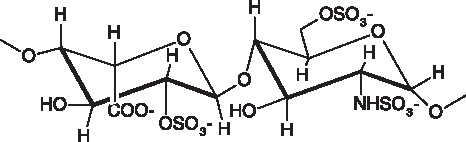
\includegraphics[width=1.0\textwidth]{gfx/background/hp_repeating_unit_structure_01.pdf}
\caption[]{
Molecular configuration of the repeating disaccharide unit of heparin (the one
which occurs most frequently in natural heparin polysaccharides). The pyranose
to the left is a 2-O-sulfated iduronic acid (IdoA2S), connected via a
1$\rightarrow$4 glycosidic linkage to the 6-O-sulfated
2-deoxy-2-sulfamido-α-D-N\-/acetylglucosamine (GlcNS6S). At physiological pH,
the charge of this disaccharide is -4 elementary charges.
}
\label{fig:bg:heparin_chemstruct}
\end{figure}

There are many more than six GAG variants with established names, such as
Chondroitin\-/6\-/sulfate (CS6), which is the same as CS4, but sulfated at the
C6 position of the galactosamine instead of in the fourth position. With the GAG
types described here so far, all major characteristics of naturally occurring
GAG molecules are covered. Other GAG types are not listed, because they are not
fundamentally different from what has been described and therefore were not
investigated in the framework of this thesis.

In organisms, all GAG chains except for HA  appear covalently bound to a core
protein, comprising a so-called \textit{proteoglycan} complex
\cite{essentials_glycobiology_gags_chapter_2009}. These large structures consist
of a linear protein with many GAGs covalently linked to it. Each GAG is linked
to the core protein via a special sugar linker, which itself is attached to
(usually) a serine residue of the core protein. As of the length of the GAG
chains, however, the biological functions of proteoglycans depend to a large
extent only on the interaction of its GAG chain(s) with other proteins, i.e.\
the free end of a GAG chain can be considered unaffected by the core protein.
This is one of the fundamental assumptions applied in this thesis project: GAGs
are considered and treated as \textit{free} molecules.


%While it is likely that their tremendous length and also their covalent linkage
%to proteoglycans serve have an overall impact on the biological function of
%GAGs, it is a valid and well-established approximation to not account for these
%facts in molecular modeling studies that aim for resolving the molecular
%mechanism of protein-GAG interaction in atomic detail... in a biological
%function and overall  treated as


\subsubsection{Pyranose conformations}
\label{background:gags:conformations}

The origin and geometry of various pyranose monosaccharide conformations is
comprehensibly classified and discussed in
\cite{classification_pyranose_conformers_1960}. The conformational nomenclature
used throughout this thesis follows IUPAC rules, which are well-described in
\cite{iupac_gag_conformations_1980}.

Free in solution, most monosaccharide rings in GAGs have one clearly predominant
conformation, and their ring structure can therefore be considered
\textit{rigid}, as is the case for e.g.\ D-glucuronic acid (GlcA), which resides
in a stable ${}^{4}\mathrm{C}_1$ chair \cite{almond_jacs_2010}. Also
N-acetyl-D-glucosamine (GlcN) mainly populates the ${}^{4}\mathrm{C}_1$ ring
conformation, which was shown to be especially stable when the GlcN becomes
sulfated \cite{Sattelle_glcnac_right_chair_2011}, as is the case in heparin. The
pyranose ring of iduronic acid (IdoA), a constituent of heparin, however, is the
only GAG pyranose that is --- free in solution, i.e.\ without any mechanical
stress --- in an equilibrium of multiple so-called ring puckers. C5 carboxyl
epimerization is the the only difference of IdoA compared to GlcA, and it
results in conformational instability. IdoA is postulated to be populated by a
mixture of mainly three conformations \cite{almond_jacs_2010}:
${}^{4}\mathrm{C}_1$, ${}^{1}\mathrm{C}_4$, and ${}^{2}\mathrm{S}_\mathrm{O}$.
Obviously, this conformational flexibility of IdoA is a \textit{structural
flexibility} which allows for different orientations of functional groups in
space, as depicted in \cref{fig:bg:idoa_conformations}.

\begin{figure}
\centering
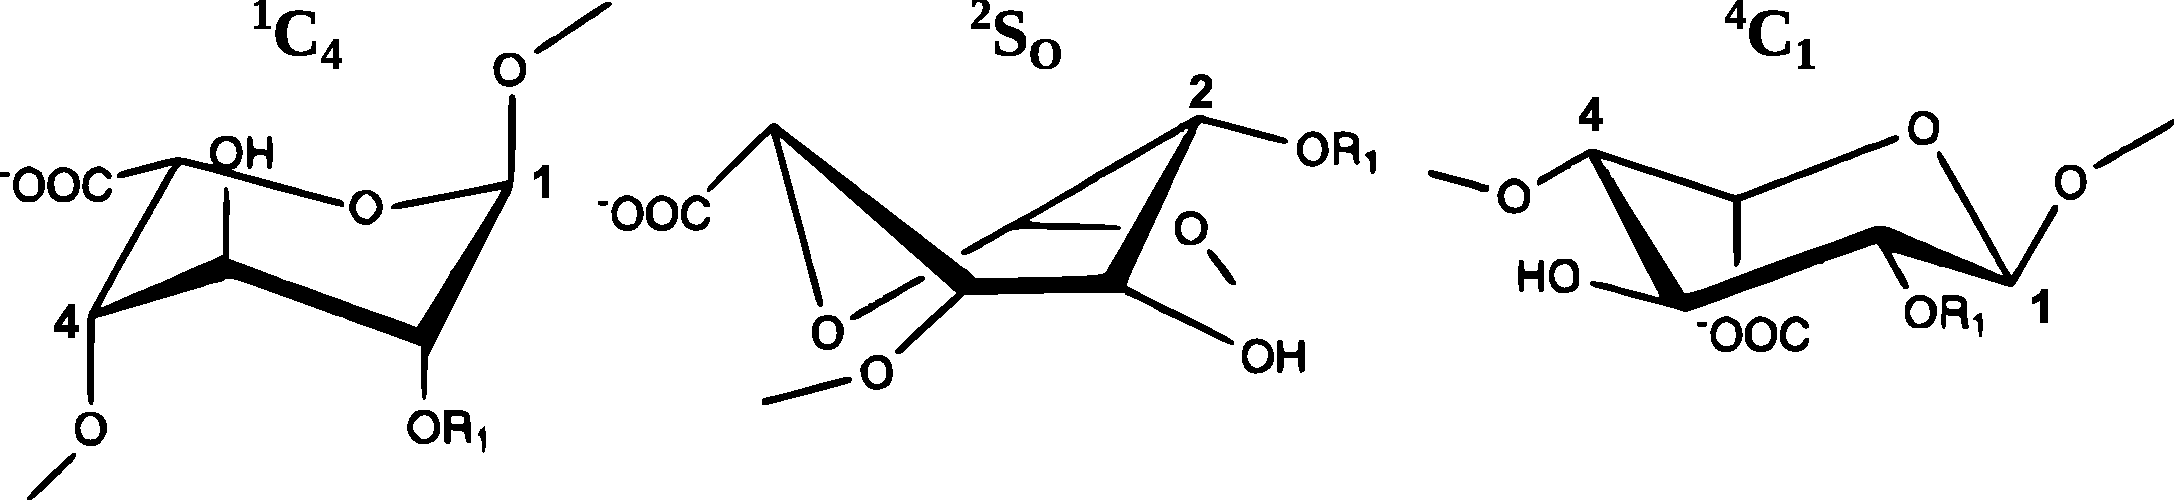
\includegraphics[width=1.0\textwidth]{gfx/background/idoa_conformations_03.pdf}
\caption[]{
The three conformations (two chairs, one skew-boat) of the pyranose L-iduronic
acid which are most populated in solution. In heparin, $\mathrm{R}_1$ is a
sulfate group.}
\label{fig:bg:idoa_conformations}
\end{figure}


The exact population ratios and exchange time scales of the conformations of
IdoA are difficult to measure and simulate \cite{almond_jacs_2010,
structure_gags_progess_perspectives_2010}, but they clearly depend on the IdoA
environment. That is, a terminal IdoA behaves differently from an IdoA pyranose
within a GAG chain. As shown by Sattelle et al., the population ratio depends on
sulfation, and IdoA2S still prevails in an equilibrium of multiple highly
populated conformations \cite{almond_jacs_2010}. Regarding heparin-internal
IdoA2S, Muñoz-García and co-workers summarize that it is in an equilibrium of
${}^{2}\mathrm{S}_\mathrm{O}$ and ${}^{1}\mathrm{C}_4$ with a negligible content
of the ${}^{4}\mathrm{C}_1$ chair \cite{conf_idoa_timeavg_restraints_2013}. The
interconversion between ${}^{2}\mathrm{S}_\mathrm{O}$ and ${}^{1}\mathrm{C}_4$
has earlier been described to exert only little geometrical change on glycosidic
linkages \cite{Mulloy_dyn_conf_heparin_2000}, rendering the overall
polysaccharide conformation independent on iduronic acid ring puckering
\cite{jin_heparin_2009}. Likewise, Gandhi and Mancera conclude that whilst the
spatial orientation of the 2-O-sulfate group in IdoA2S in heparin is altered
during conformation interconversion, no significant structural change can be
seen in the backbone of the polysaccharide chain \cite{gandhi_structure_2008}.


\subsubsection{General aspects about protein-GAG interaction}

It is state of knowledge that GAGs play a critical role in many biological
processes \cite{handel_2005}. In many of these scenarios, GAGs directly and
\textit{specifically} interact with proteins on the molecular level
\cite{prot_gags_glycomics_review_2006}. According to Esko and Linhardt, more
than 100 GAG-binding proteins have been described in literature
\cite{essentials_glycobiology_protgags_2009}. To a large extent, the
corresponding studies were focused on protein interaction with heparin only.
Esko and Linhardt speculate that this bias towards heparin may reflect the
commercial availability of heparin and the fact that the interaction between
proteins and heparin can be assumed to properly mimic the physiological
interaction of proteins with heparan sulfate, which is especially abundant on
cell surfaces and in the extracellular matrix. Esko and Linhardt note that
relatively few proteins are known to interact with chondroitin sulfate or
keratan sulfate. However, in some cases, especially chondroitin sulfate's
interaction with proteins may be physiologically relevant, because chondroitin
sulfate is the most abundant GAG in the body
\cite{gandhi_structure_2008} and available in many tissues
\cite{essentials_glycobiology_protgags_2009}.

Several protein-GAG systems of which it is long known that they have huge
biological impact were, in the course of countless studies, investigated via
structural biology methods, biochemically, and via molecular modeling approaches
in order to understand the \textit{molecular basis} of the interaction.
Fundamental findings were especially made with X-ray crystallography and via
nuclear magnetic resonance (NMR), both of which are able to spatially resolve
the arrangement of atoms in the bound state of a protein-GAG complex. However,
NMR and X-ray studies implicate an enormous experimental effort and are often
not successful, so that up to now the number of experimentally obtained
protein-GAG complex structures deposited in the PDB is still quite low (about
85 as of today).

% Still, from these well-investigated complexes, a number of
% essential observations is to be made for this thesis work.

\nomenclature{dp}{degree of polymerization}

The experimentally resolved structures of protein-GAG complexes typically
contain GAG molecules of lengths between dp2 and dp10, with the most common
length being dp5 (\enquote{dp} stands for degree of polymerization, and the
following number is the number of monosaccharides in the molecule). Khan et al.\
argue that HP dp4 possesses a sufficient number of at least six sulfate groups
and two carboxyl groups to generate protein specificity for heparin
\cite{semi_rigid_heparin_structures_2010}. Hence, GAG binding epitopes
responsible for affinity \textit{and} specificity of the protein-GAG interaction
are typically rather short --- at least for the systems contained in the PDB so
far, and a counter-example is yet to be discovered. Likewise, recent
experimental and molecular modeling studies for the investigation of protein-GAG
systems focused on using short GAGs \cite{pichert_characterization_2012,
hintze_sergey_2014, gandhi_coombe_2008, Gandhi01102009,
mancera_gandhi_jcim_2011, agostino_mancera_gandhi_2014}. An important
observation is that in most crystal structures, GAG binding sites are found on
surface-exposed positions, almost always containing positively charged amino
acid residues (at physiological pH, which are arginine and lysine).

Regarding heparin-protein interaction, a number of crystal structures and NMR
experiments suggest that when heparin binds to a protein, the iduronic acid may
undergo an induced fit, and prefer one of its possible ring conformations
\cite{gandhi_structure_2008}. The conformational flexibility of IdoA and
therefore its ability to structurally adjust itself to a protein may be one of
the reasons why many important and high-affinity protein-GAG interactions
involve heparin, and not other GAG types. On the other hand, there are also
protein-GAG complexes for which it has been shown that IdoA in the bound state
can still assume multiple conformations \cite{barbero_jacs_2005}, in which case
the entropy penalty associated with the restriction of single degrees of freedom
would be reduced. Overall, however, the scientific community generally assumes
that heparin's pure charge density is mainly responsible for its seemingly
dominant role in protein-GAG interaction \cite{gandhi_structure_2008,
essentials_glycobiology_protgags_2009}.



\subsubsection{Structure of GAGs}

While the geometry of monosaccharides is well-investigated and in most of the
cases known with an enormous degree of detail, the investigation of the
three-dimensional solution structure of GAG polysaccharides, i.e.\ its overall
flexibility and conformation, is rather unclear and topic of ongoing research
\cite{structure_gags_progess_perspectives_2010}. The GAG structures contained in
the PDB, as stated above, are limited to smaller fragments of not more than 10
monosaccharides. Among these bound structures, GAGs appear to be linear, quite
flexible molecules that do not assume a special secondary structure.
Additionally, Khan et al.\ found via X-ray scattering and constrained modeling
that longer heparin oligosaccharides (up to dp36) that are free in solution
assume a rather extended semi-rigid conformation
\cite{semi_rigid_heparin_structures_2010}. One of the most important criteria
for characterizing GAG structures are their glycosidic linkage dihedral angles.
In this regard, the X-ray and NMR measurements reported in literature very much
agree on a certain angle interval, which is accessible to all major GAG types,
conceptually comparable to the well-known backbone dihedral angle intervals
which are valid for proteins. Obviously, this kind of data enables us to
estimate whether a certain GAG structure is valid or not, and it also allows us
to quantify the overall backbone flexibility of GAGs. An overview over
literature-reported heparin backbone dihedral angles can be found in e.g.\
\cite{semi_rigid_heparin_structures_2010}.


\section{Interleukin-10 (IL-10)}

\subsection{A primer on the biological relevance of IL-10}

The biological relevance of the cytokine IL-10 has extensively been reviewed in
the work of Moore et al. \cite{moore_2001}. Via its ability to inhibit effector
functions of T cells, monocytes, and macrophages, its critical
\textit{in vivo} function is to limit and eventually terminate inflammatory
responses. The prime evidence in this regard are IL-10-deficient mice which show
exaggerated innate immune responses and rather spontaneously develop
inflammatory bowel disease \cite{mueller_il10defmouse_1993,
roers_il10_mice_2004,rubtsov_il10_mice_2008}. In this context, it is notable
that IL-10 is highly conserved among different species
\cite{il10_dna_rabiit_2000, porcine_il10_1995}. Specifically, the sequence
identity between murine and human IL-10 is \SI{73}{\percent}, with no artificial
alignment being required. The residue conservation between murine an human IL-10
is visualized in
\cref{fig:bg:murine_human_il10_sequence}.

\begin{figure}
\centering
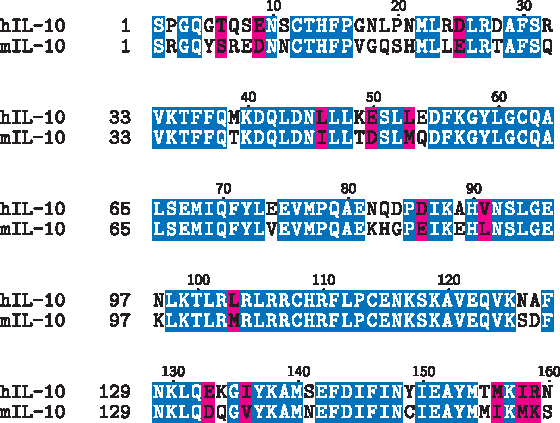
\includegraphics[width=0.7\textwidth]{gfx/background/murine_human_Il10_alignment_01.pdf}
\caption[]{
Conservation of the amino acid sequences among human and murine IL-10 (UniProt
\cite{TheUniProtConsortium01012014} identification codes P22301 and P18893,
respectively). 117 out of 160 amino acid residues are identical (blue), 12 are
similar (magenta), and all other residues are not conserved. The sequence
identity and similarity are \SI{73}{\percent} and \SI{88}{\percent},
respectively. The sequences are naturally well-aligned, ClustalW
\cite{clustalw_2008} could not optimize the alignment. The figure was created
using Strap \cite{strap_website}.}
\label{fig:bg:murine_human_il10_sequence}
\end{figure}




While protective on the one hand, immune responses have the potential to
destruct not only pathogens but also host cells, and hence are a major threat to
the integrity of host tissues. Therefore, a tight regulation of immune responses
is crucial for keeping the fine balance between immunopathology and
immunosuppression, and IL-10 is one of only a few cytokines being pivotal for
down-regulating immune responses. Sabat et al.\ summarize that IL-10's special
physiological relevance lies in the prevention and limitation of over-whelming
specific and unspecific immune reactions and, in consequence, of tissue damage
\cite{sabat_bio_il10_review_2010}. Saraiva and O'Garra conclude that the absence
of IL-10 can not always be compensated by other regulatory mechanisms,
indicating a \textit{non-redundant} role for IL-10 in limiting inflammation
\cite{saraiva_ogarra_2010}. However, despite the observed anti-inflammatory
effects of IL-10, the attempts to use it directly as a therapeutic agent in
various inflammatory conditions yielded disappointing results
\cite{il10_therapy_review_2003}. The IL-10 system turned out to be more complex
than initially assumed, and it was found that its functions largely depend on
its micro-environment, i.e.\ the cells producing the cytokine
\cite{roers_mueller_2008}, the cells responding to them, and the specific immune
environment in which it is released \cite{mosser_il10_newperspectives_2008}.
Furthermore, it was found that IL-10 also has pro-inflammatory effects in
certain conditions \cite{lauw_il10_proinflamm_2000}, pointing towards an
incredibly multifaceted role of IL-10 in biology. Likewise, IL-10 is often
called a \textit{pleiotropic} cytokine. Overall, IL-10 is a crucial regulator of
immune responses, and, as Sabat et al.\ conclude, knowledge regarding IL-10
effects forces us to think about modulation of IL-10 activity as a potential
therapy \cite{sabat_bio_il10_review_2010}. A comprehensible and extensive review
about strategies for the usage of IL-10 in human disease has been published
by O'Garra et al. \cite{il10_disease_strategies_ogarra_2008}.


\subsection{IL-10 and its biological relation to GAGs}

As a regulator of inflammation, IL-10 plays a major role in tissue repair. Roers
et al.\ found in animal studies that down-regulation of IL-10 affects the repair
process and has an impact on the resulting tissue --- IL-10-deficient mice
showed a significantly enhanced re-epithelialisation and skin contraction,
suggesting that the local inflammatory response to tissue injury promotes the
repair process \cite{roers_il10mice_woundhealing_2007}. Especially in defects
and wound healing scenarios, larger concentrations of IL-10 are traveling the
space between cells for exerting IL-10's major biological effects. As of the
abundance of GAGs in tissue, in particular on cell surfaces and within the
extracellular matrix (ECM), it is a valid question to ask how GAGs might
regulate the function of IL-10 --- as of the fine balance that is required to be
maintained in regulating immune responses, even a slight modulation of IL-10
function via ECM components might be of biological significance.

The central work motivating this thesis project has been published back in 2000
by Salek-Ardakani et al.\ \cite{salek_ardakani_2000}, who have shown
experimentally that

\begin{itemize}
\item IL-10 binds HP and HS with a $\mathrm{K}_\mathrm{D}$
value in the nanomolar range (via affinity chromatography and surface plasmon
resonance).
\item soluble HP and HS inhibit IL-10-induced expression of CD16 and CD64 in a
concentration-dependent manner (via \textit{in vitro} peripheral blood
mononuclear cell proliferation experiments).
\item a reduction of sulfated proteoglycans at the cell surface negatively
affects the IL-10-induced expression of CD16 and CD64.
\end{itemize}

Hence, in these experiments, IL-10 was found to bind GAGs quite strongly and
evidence was obtained for GAGs being able to modulate IL-10 function: soluble
GAGs were shown to \textit{inhibit} the biological activity of IL-10, whereas
the reduction of the sulfation of cell-surface proteoglycans was shown to reduce
IL-10 function, i.e.\ cell-surface-attached \textit{sulfated} GAGs may
\textit{enhance} IL-10 function, possibly because they facilitate the
interaction between IL-10 and its transmembrane receptors.

Unfortunately, the clear results obtained by Salek-Ardakani et al.\ have so far
not been reproduced and published elsewhere in a different context, rendering
their work (\cite{salek_ardakani_2000}) to be the only point of support when it
comes to prove the ability of GAGs to modulate IL-10 function. Notably, in their
experiments, the HP concentrations required to inhibit IL-10 function by more
than \SI{50}{\percent} was quite large, with about
\SI{0.5}{\milli\gram\per\milli\liter}. Such a high concentration may be
responsible for side effects not occurring under physiological conditions.
Furthermore, the fact that polymeric high molecular weight GAGs from animal
sources (all provided by the same commercial vendor) were used in the
experiments makes it difficult to assess the effects of GAG \textit{length} and
\textit{impurity} on the results. Still, even considering these sources of
error, the results published by Salek-Ardakani et al.\ are rather convincing,
and, as they conclude, these findings support the hypothesis that soluble and
cell-surface GAGs and, in particular, their sulfate groups are important in
modulation of IL-10 activity, and further studies are required to identify the
molecular mechanism of GAGs binding to IL-10. Up to now, several years later, no
structural details about IL-10-GAG interaction have been published, and the
deeper biological meaning of IL-10-GAG interaction is still not clarified.

However, it is often speculated that the major role of cytokine-GAG interaction
in general could be the ability of the ECM to affect the diffusion of such
cytokines, and therefore affect their location and local concentration. In his
review of cytokine-GAG interaction, Coombe notes that it was postulated that the
interaction of cytokines with their receptors evolved \textit{independently} of
GAG binding, with GAG binding being an additional feature that localizes
cytokines within tissues \cite{coombe_cytokine_gag_2008}. In any case, the
investigation of the molecular interaction between IL-10 and GAGs will provide
further insights about the relevance and the mechanism of this interaction.


\subsection{Structure of the IL-10 system}

\subsubsection{General aspects}
Shortly after the biological relevance of IL-10 had been discovered (reviewed in
1993 by Moore and O'Garra \cite{il10_first_review_1993}), huge efforts were
undertaken to resolve the three-dimensional structure of the protein itself and
of its receptors, especially by the groups of Zdanov and Walter
\cite{zdanov_review_2010, zdanov_review_2004, bookchapter_walter_il10_2004}.
From early investigations, it was clear that IL-10 is a \textit{homodimeric}
protein, comprised of two equivalent and rather short polypeptide chains of 160
amino acids each, and with a high helical content
\cite{vieira_moore_il10homodimer_1991}. The first IL-10 structures obtained via
X-ray crystallography were independently published in 1995 by Zdanov et al.\
\cite{Zdanov1995}, and by Walter et al.\ \cite{il10_crystal_walter_1995}, and
they were in agreement, considering the resolution capacity of the experiments.
In 1996, Zdanov et al.\ published another crystal structure of IL-10
\cite{Zdanov1996}. With a spatial resolution of \SI{1.6}{\angstrom} it is the
best-resolved structure of IL-10 published to date, and contains all amino acid
residues except for the first five N-terminal ones. This structure had been
deposited in the PDB with identification code 2ILK and was used throughout this
thesis project whenever it was required to represent the IL-10 structure --- for
visualization purposes, and for \textit{in silico} experiments.

\begin{figure}
\centering
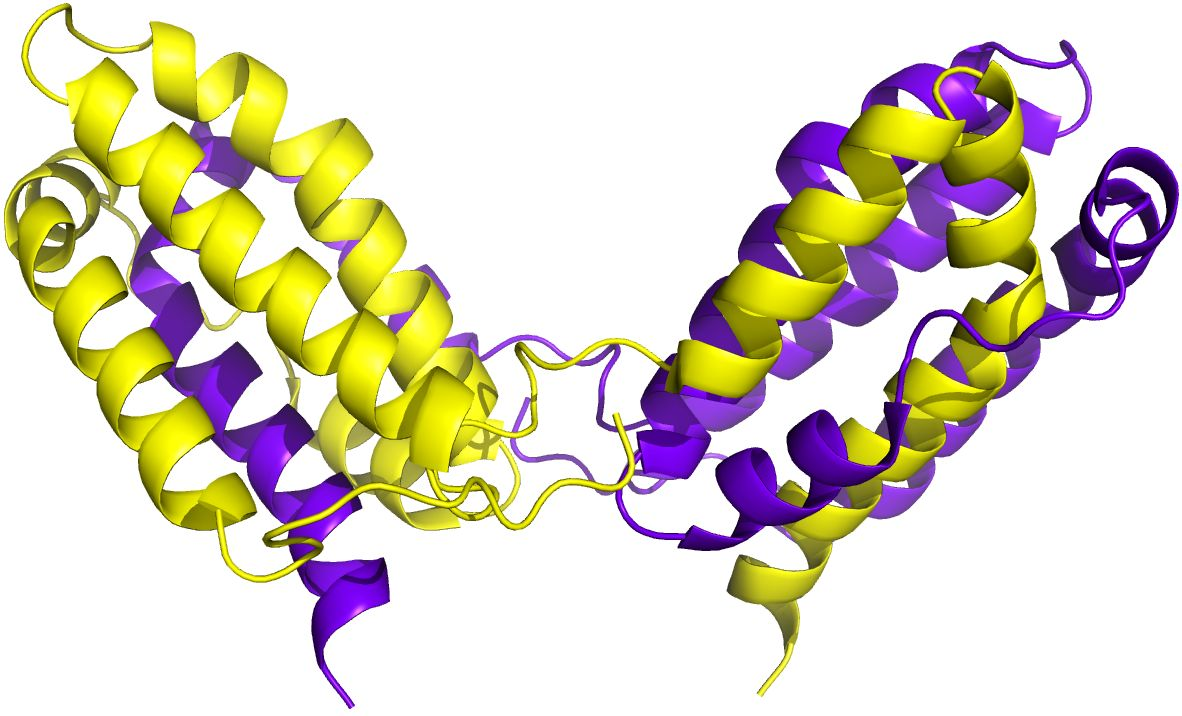
\includegraphics[width=1.0\textwidth]{gfx/background/IL10_2ilk_dimer_yellow_blue.jpg}
\caption[]{
Structure of human IL-10 according to PDB entry 2ILK (obtained via X-ray
crystallography, with a spatial resolution of \SI{1.6}{\angstrom}
\cite{Zdanov1996}) in cartoon representation, created with PyMOL \cite{pymol}.
The figure shows the IL-10 homodimer (which is the predominant form of IL-10 in
solution), made of two equivalent intertwined IL-10 monomers. One monomer is
shown in yellow, the other monomer is shown in purple. The dimer has two
structural domains, and each monomer contributes four helices to one domain, and
two helices to the other domain. The two domains are related by a two-fold
(\SI{180}{\degree}) rotational symmetry. From the point of view shown here, it
becomes obvious why IL-10 is sometimes described to have a \enquote{V-shape}.
}
\label{fig:bg:il10_dimer_vshape}
\end{figure}

\subsubsection{Structure description}

Under physiological conditions in solution, IL-10 has been shown to
predominantly exist as a \textit{homodimer} --- the population of the monomeric
form is negligible and not biologically active \cite{syto_il10_homodimer_1998}.
In literature, the name IL-10 refers to the biologically active dimeric form of
the protein. The crystal structure of the IL-10 homodimer (according to PDB
entry 2ILK) is visualized in \cref{fig:bg:il10_dimer_vshape}. IL-10 is a
so-called \enquote{intertwined} or \enquote{intercalated} dimer of two sub-units
(the monomers), each consisting of six helices, named A-F. The IL-10 dimer has
two structural domains, and each monomer contributes four helices to one domain,
and two helices to the other domain (for clarity, this is color-encoded in
\cref{fig:bg:il10_dimer_vshape}). Each of both six-helix domains is comprised of
helices A-D of one monomer, together with helices E' and F' of the other
monomer. The two monomers are intertwined in a perfectly symmetric way,
resulting in a \SI{180}{\degree} (two-fold) rotational symmetry by which both
domains of the IL-10 homodimer are related. Considering the point of view shown
in \cref{fig:bg:il10_dimer_vshape}, the overall shape of IL-10 is sometimes
equated to the letter V and therefore called \enquote{V-shape}, which I adopt in
this thesis.

\begin{figure}
\centering
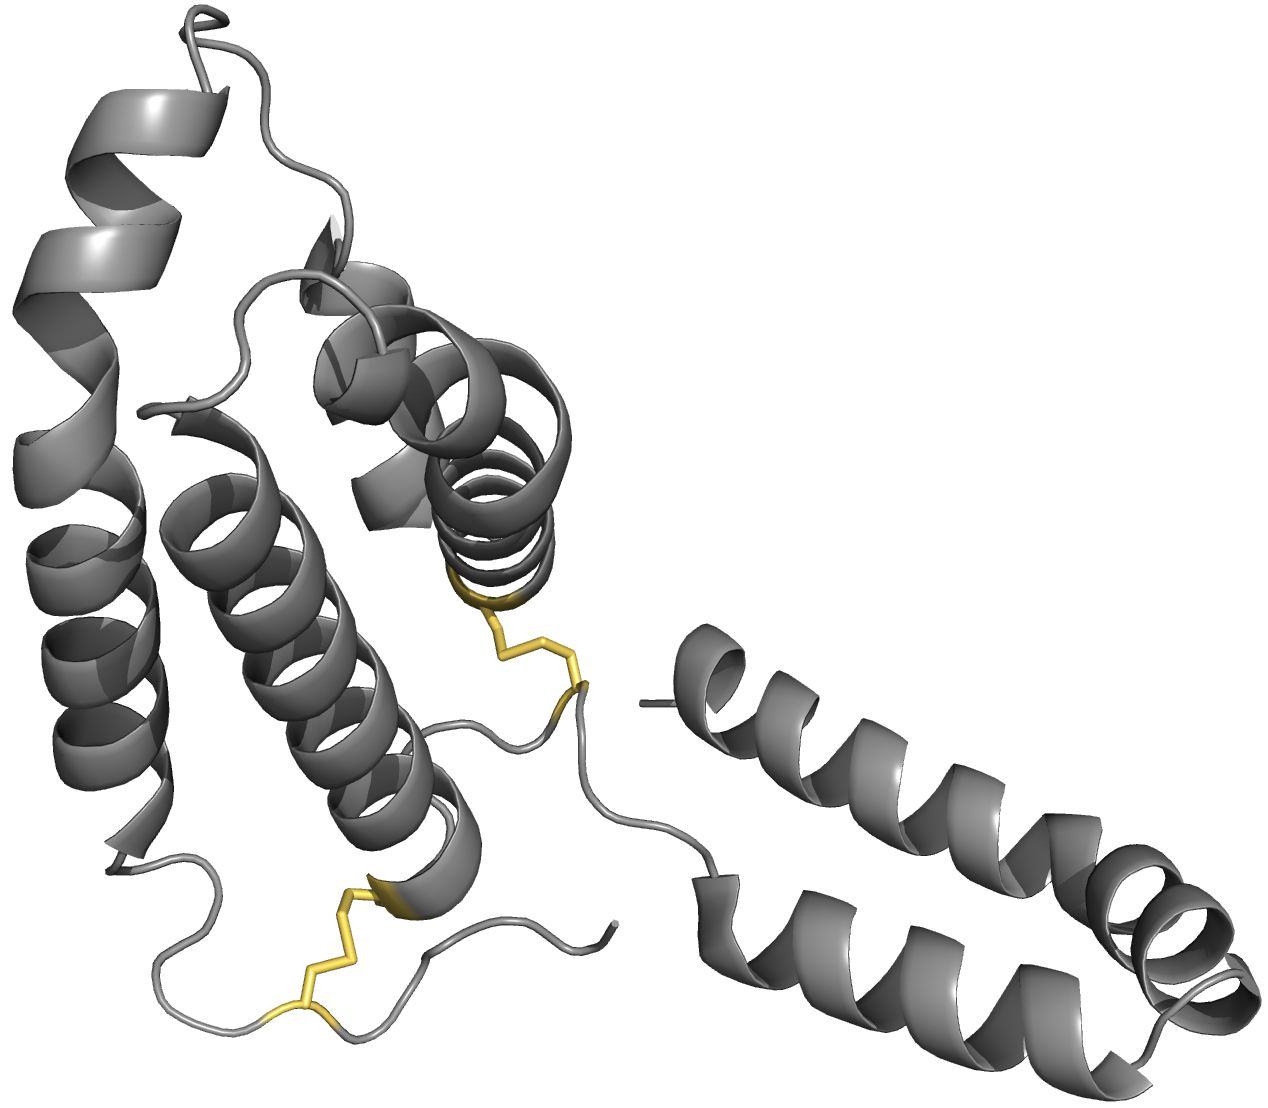
\includegraphics[width=0.7\textwidth]{gfx/background/IL10_2ilk_disulfide_with.jpg}
\caption[]{
Structure of the human IL-10 monomer, as extracted from the homodimeric
structure with PDB code 2ILK \cite{Zdanov1996}, in cartoon representation. In
the homodimeric structure, the four-helix bundle to the left builds a domain
together with the two-helix bundle from a second IL-10 monomer. The structure of
the monomer is stabilized by two disulfide bridges, shown here in yellow. }
\label{fig:bg:il10_monomer_disulfide}
\end{figure}

The structure of the IL-10 homodimer is stable. First of all, each monomer has
approximately \SI{85}{\percent} helical content \cite{Zdanov1995}. Secondly, the
structure of each monomer is stabilized by two intramolecular disulfide bridges,
as shown in \cref{fig:bg:il10_monomer_disulfide}. Furthermore, the
interpenetration of the two monomers is tight, and the resulting domain
structure is stabilized by the formation of a large interhelical hydrophobic
core with many hydrogen bonds. Zdanov summarizes that only eight hydrophobic
residues out of 66 in the ordered part of IL-10 do not participate in the
formation of the hydrophobic core \cite{Zdanov1995}. However, whereas the two
six-helical domains are rigid for named reasons, and are unlikely to change
their conformation upon external stress, the junction between both domains,
i.e.\ the groove of the V-shape, bears the potential for some hinge-like
flexibility \cite{Zdanov1995}. Also, according to Zdanov, the N-terminal
residues 1-5 (which were not resolved in the crystal structure 2ILK)
\enquote{are disordered and probably turn away from the interdomain interface
and assume multiple conformations in solvent} \cite{Zdanov1996}.


\subsubsection{IL-10 and its receptors}


\vspace{0.5cm}
\textit{\textbf{IL-10 signaling requirements.}}
In the course of many studies it has been found that two receptor proteins are
required for IL-10 to exhibit its biological function: the primary high affinity
receptor IL-10R1 and the secondary low affinity receptor IL-10R2
\cite{mosser_il10_newperspectives_2008}. The established model in literature is
that IL-10 \textit{first} binds to the transmembrane receptor IL-10R1, which
itself is associated with the Janus tyrosine kinase Jak1. Subsequent binding of
IL-10R2 to the intermediate IL-10/IL-10R1 complex recruits the kinase Tyk2,
which initiates a cascade of signal transduction events that include tyrosine
phosphorylation of Jak1 and Tyk2, trans-phosphorylation of both IL-10 receptor
chains, and activation and nuclear translocation of the transcription factor
STAT3
\cite{donnelly_finbloom_il10_1999}. The idea that ternary complex formation
occurs in a sequential fashion, whereas IL-10/IL-10R1 binding is required for
the ternary complex IL-10/IL-10R1/IL-10R2 to form has been supported by a study
of Yoon et al. that suggested that IL-10/IL-10R1 binding triggers a
conformational change in a couple of IL-10 residues important for IL-10R2
binding \cite{il10r2_conf_changes_2006}.

As described above, the IL-10 homodimer has \textit{two} equivalent six-helical
domains. In various original publications and in recent reviews about the IL-10
system it is suggested or even presented as common knowledge that a large
ternary complex is \textit{required} for signaling, involving \textit{both}
domains of the IL-10 dimer, two IL-10R1 molecules, and two IL-10R2 molecules
(\enquote{IL-10 signals through a two-receptor complex consisting of two copies
each of IL-10R1 and IL-10R2} \cite{mosser_il10_newperspectives_2008},
\enquote{Functional IL-10 receptor complexes are tetramers consisting
of two IL-10R1 polypeptide chains and two IL-10R2 chains.}
\cite{donnelly_finbloom_il10_1999}, \enquote{The IL-10 receptor complex on cells
is composed of four transmembrane polypeptides: two chains of IL-10R1 that bind
ligand and two chains of IL-10R2 that initiate signal transduction}
\cite{pestka_2004_il10_receptors_review}). However, Josephson et al.\ published
in year 2000 that the interaction of \textit{one} domain of the IL-10 homodimer
with \textit{one} molecule of IL-10R1 and \textit{one} molecule of IL-10R2 is
\textit{sufficient} for activation of the intracellular kinases Jak1 and Tyk2,
i.e.\ for cellular responses to IL-10 \cite{il10_monomer_2000}, and their
experimental procedure and conclusions are rather convincing. Being sure about
the minimal molecular system required for triggering IL-10 function is
especially important to keep in mind when considering artificial modulation of
the IL-10 system.

\vspace{0.5cm}
\textit{\textbf{Primary receptor IL-10R1.}} The X-ray crystal structure of the
IL-10 homodimer in complex with the extracellular domain of its high affinity
transmembrane receptor IL-10R1 has been published in 2001 \cite{Josephson2001}
and deposited in the PDB with identification code 1J7V. It has a spatial
resolution of \SI{2.9}{\angstrom}, and revealed that IL-10R1 binds to the
\enquote{sides} of the IL-10 V-shape, as depicted in
\cref{fig:bg:il10_il10r1_complex}.

\begin{figure}
\centering
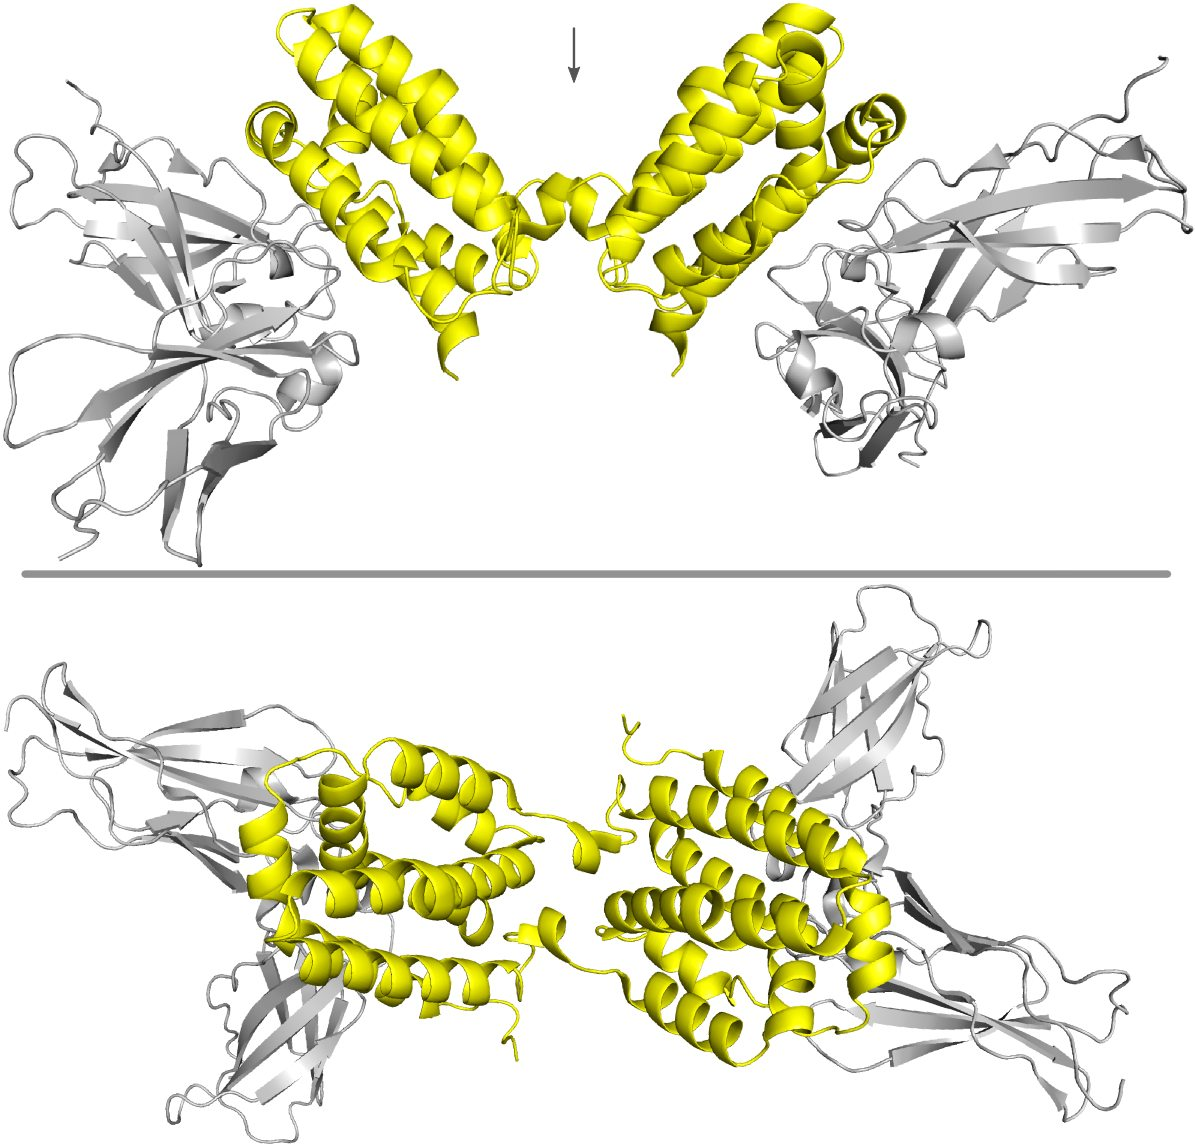
\includegraphics[width=1.0\textwidth]{gfx/background/il10r1_il10_complex_topside_02.jpg}
\caption[]{
Structure of the human IL-10 homodimer (yellow) in complex with the
extracellular domain of its high affinity transmembrane receptor IL-10R1 (gray),
both in cartoon representation, according to PDB entry 1J7V (obtained via X-ray
crystallography, with a spatial resolution of \SI{2.9}{\angstrom}
\cite{Josephson2001}). The top panel shows IL-10 from the same point of view as
used in \cref{fig:bg:il10_dimer_vshape}, i.e.\ it shows the \enquote{front/back}
direction of the V-shape. The bottom panel shows the V from the
\enquote{top-to-bottom} perspective, as indicated with the small arrow in the
top panel. In this terminology, the IL-10R1 molecules bind to the
\enquote{sides} of the V. Although two IL-10R1 molecules are shown in the
figure, their binding to IL-10 is independent, and only one IL-10R1 molecule is
required for triggering the IL-10 signal cascade.}
\label{fig:bg:il10_il10r1_complex}
\end{figure}

According to the principal authors of the crystal structure, about 27 residues
from IL-10 make contact with IL-10R1. These residues are mostly polar, and
divided into two structurally distinct interaction surfaces, both on the side of
the IL-10 V-shape. A deeper structural characterization of the interaction
between IL-10 and IL-10R1 can be found in the work of Josephson et al.
\cite{Josephson2001}, and in a comprehensive book chapter on the structural
properties of the IL-10 system by Walter \cite{bookchapter_walter_il10_2004}.


\vspace{0.5cm}
\textit{\textbf{Secondary receptor IL10-R2.}}
IL-10R2, the secondary low affinity transmembrane receptor of IL-10, is a
\textit{shared} receptor among the so-called IL-10 family of cytokines: besides
for IL-10, it serves as a receptor for IL-22, IL-26, and IFN-$\lambda$
\cite{zdanov_review_2010}. The scientific community was so far not able to
crystallize the entire ternary complex of the IL-10 system. That is, despite of
certain modeling efforts, the structure involving the IL-10 homodimer as well as
IL-10R1 and IL-10R2 in a single complex has not been determined with all
certainty up to now. Also, so far no other ternary complex structure from the
IL-10 family of cytokines involving IL-10R2 has been published. However, in
2010, the crystal structure of the extracellular domain of IL-10R2 alone was
published by Yoon et al. \cite{il10r2_structure_2010}. It has a resolution of
\SI{2.1}{\angstrom} and was assigned the PDB identification code 3LQM.


\vspace{0.5cm}
\textit{\textbf{Ternary complex (IL-10 + IL-10R1 + IL-10R2) model.}}
Before 2012, various different (and contradictory) models of the ternary IL-10
signaling complex were published, most of them based on rational positioning
using the input of certain experimental data, and sometimes using \textit{in
silico} molecular modeling techniques \cite{zdanov_review_2010, Josephson2001,
yoon_samestructdifffct_2005, il10r2_conf_changes_2006, il10r2_structure_2010}.


\begin{figure}
\centering
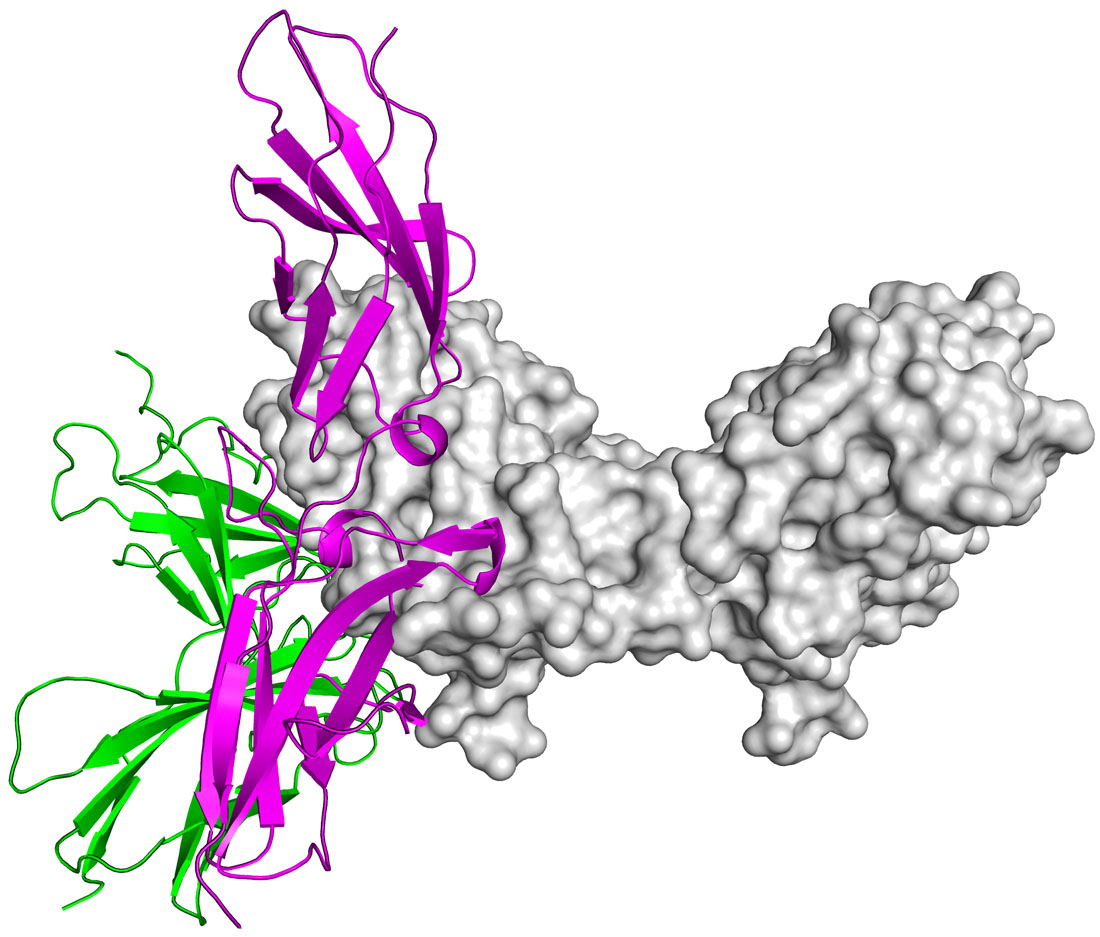
\includegraphics[width=1.0\textwidth]{gfx/background/il10dimer_surface_r1cartoon_r2cartoon_front_06_small.jpg}
\caption[]{
Model of the ternary IL-10 signaling complex with the IL-10 homodimer shown in
gray surface representation, and IL-10R1 (green) and IL-10R2 (magenta) shown in
cartoon representation. The single structures are taken from PDB entries 2ILK
(IL-10), 1J7V (IL-10R1), and 3LQM (IL-10R2). The relative positioning of the
three molecules is based on the recently published structure of the ternary
IL-20/IL-20R1/IL-20R2 complex (PDB 4DOH \cite{logsdon_il20r2compl_2012}), and
has been derived in a simple structural alignment procedure.}
\label{fig:bg:il10_il10r1_il10r2_model}
\end{figure}

In 2012, the crystal structure of the ternary IL-20/IL-20R1/IL-20R2 complex was
published by the Walter group and deposited in the PDB under the access code
4DOH \cite{logsdon_il20r2compl_2012}. This is the first publicly known ternary
complex structure in the IL-10 family of cytokines. It seems obvious that an
alignment of IL-10 system components onto the corresponding molecules of the
IL-20 system provides one of the most reliable models for the geometrical
arrangement of molecules in the ternary IL-10 system. Since this has not been
published and discussed in literature so far, I have created this rather simple
model, using rudimentary structural alignment tools as implemented in PyMOL
\cite{pymol}. Specifically, I have first aligned the entire ternary IL-20 system
(4DOH) onto the IL-10/IL-10R1 complex (1J7V) via alignment of IL-20R1 onto
IL-10R1. Both R1 molecules are structurally highly similar, with a C-$\alpha$
RMSd of \SI{2.2}{\angstrom}. In a second step, I have aligned the IL-10
homodimer (2ILK) onto IL-20 of the 4DOH system. IL-20 is structurally similar to
a single six-helical domain of IL-10, yielding a C-$\alpha$ RMSd of
\SI{3.3}{\angstrom}. Lastly, I have aligned IL-10R2 (3LQM) onto IL-20R2 of the
4DOH system. The global geometry of IL-20R2 and IL-10R1 is very similar, but due
to significant differences in various loops and interdomain angles, the
C-$\alpha$ RMSd after alignment of both molecules is \SI{6.3}{\angstrom}. The
resulting model is depicted in \cref{fig:bg:il10_il10r1_il10r2_model}. In
summary, it contains the IL-10 homodimer structure from PDB entry 2ILK, the
IL-10R1 structure 1J7V, and the IL-10R2 structure 3LQM. While this simple model
should not be taken literally on the scale of single atomic contacts, the
overall global positioning of molecules with respect to each other likely
matches that of the naturally occurring ternary IL-10 signaling complex.
Therefore, it can serve to give an impression about GAG molecule binding
locations that could potentially interfere with receptor binding.


\section{Aim and scope of this thesis}

Co-crystals of protein-GAG complexes are difficult to obtain, since GAGs feature
a high degree of conformational flexibility and biologically relevant
protein-GAG complexes are not always characterized by  high binding affinity.
NMR assignments of longer oligosaccharides are complicated or impossible to
obtain due to their repetitive nature. Furthermore, chemical synthesis of
oligosaccharides is very difficult. In short, the systematic experimental
investigation of protein-GAG systems is highly challenging and resource
intensive. In the past, important advanced have been made in the field of the
\textit{computational} investigation of these systems, with pioneering work
performed especially by the groups of Mancera and Imberty
\cite{imberty_perez_protgag_comp_book_2006, imberty_gag_prot_carbres_2007,
gandhi_structure_2008}. One of the reasons why \textit{in silico} investigations
of protein-GAG systems can be of particularly large value is the conceptually
straight-forward representation of arbitrary GAG molecules in simulation
systems. Also, as known from other fields of research, the effect of amino acid
mutations on a certain receptor-ligand system, for instance, can often reliably
be described using modern \textit{in silico} simulation approaches. An
interesting work highlighting the importance of combining experimental and
theoretical approaches in order to obtain a clearer understanding of the
molecular recognition properties of protein-GAG systems has been published by
the group of Prof. Huster at the University Leipzig in collaboration with our
group, about the molecular mechanism of the IL-8-GAG interaction
\cite{pichert_characterization_2012}.

Motivated by the encouraging groundwork done in the field of \textit{i)}
experimental IL-10-GAG system investigation and \textit{ii)} the \textit{in
silico} investigation of protein-GAG systems in general, the aim of this project
is to unravel atomic details of IL-10-GAG interaction with theoretical and
computational means. Furthermore, since the \textit{in silico} methods for
protein-GAG investigation are still in their infancy, this thesis project
included from the beginning, if required, the development and improvement of
methodological approaches. From the beginning of the project onwards, it was the
plan to at some point integrate \textit{in silico}-based predictions with
experimental results from collaborators at Prof. Huster's laboratory in Leipzig.
The ultimate goal was to be able to provide insights into the mechanisms
determining IL-10-GAG interaction. Furthermore, methodology developed during
this project should be applicable to protein-GAG systems in general, rendering
it valuable for a large field of research.

Specifically, one of the first questions to be answered in this project was
where on the IL-10 homodimeric surface GAGs could potentially bind. Based on
such information, a subsequent fine-grained investigation should identify all
special determinants of IL-10-GAG interaction with atomic detail. For instance,
two important questions are whether there are certain key amino acid residues in
IL-10 that are especially relevant for GAG binding or whether there is binding
specificity of IL-10 for certain GAGs. The ultimate goal of this project was to
clarify the molecular mechanism of IL-10-GAG interaction and its possible
implications for IL-10's biological function. A resulting vision would then be
to be able to gain control over IL-10 function within artificial extracellular
matrices for improved tissue regeneration.

This research is in line with studies on cytokine-GAG interaction performed
earlier in other groups, such as the experimental investigation of IL-2-GAG
interaction, by which strong evidence was found that binding of HP and HS to
IL-2 happens, but does not interfere with IL-2/IL-2 receptor interaction
\cite{il2_gags_rider_1997}. In further studies, the authors concluded that
the IL-2-GAG interaction may be a mechanism for retaining the cytokine in an
active form close to its site of secretion in the tissue, an thus supporting the
paracrine role of IL-2 \cite{il2_gags_1998}. Also in case of IL-5 it was found
that it binds HP and HS and that it may modulate its biological function
\cite{il5_gags_coombe_1998}. The authors speculate that the manufacture of a
synthetic GAG or an analogue that binds IL-5 and prevents its localization to
biologically responsive tissue sites could enable the development of a new
approach to controlling diseases. Furthermore, IL-7 was found to bind to HP and
HS, and the authors speculated that HP may act as a carrier for IL-7, blocking
its interaction with target cells and protecting it from degradation during
transit \cite{il7_gags_1995}.

%- Motivation and goal: investigate IL-10-GAG system with computational
%      methods, in collaboration with...


\section{In-silico methods for investigating protein-GAG interaction}

%\subsubsection{GAG structures used in \textit{in silico} experiments}

\subsubsection{GAG representation approximations: isolation, length, purity}

As has been stated in \cref{background:gags}, one of fundamental assumptions
applied in this thesis project is that GAGs are treated as \textit{free}
molecules.

%While it is likely
%that their tremendous length and also their covalent linkage to proteoglycans
%serve have an overall impact on the biological function of GAGs, it is a
%valid and well-established approximation to not account for these facts in
%molecular modeling studies that aim for resolving the molecular mechanism of
%protein-GAG interaction in atomic detail... in a biological function and overall  treated as

A more severe approximation applied in this thesis is the treatment of GAGs as
\textit{short} molecules. Considering the  mostly ranging from tetra- to hexasaccharides. Considering the level of atomic detail aimed for ... to be observed... in this
thesis project, GAGs are modeled as short molecules.


Also, when treating GAGs as short molecules, they are represented by the ideal
periodic repetition of the most frequently observed disaccharide unit,
impurities or variations in the monosaccharide sequence are ignored.

ir ideal periodic

explain DP, degree of polymerization



From Sergey: Computationally, GAG containing systems are still very challenging
to handle because of their high flexibility as it applies for saccharides in
general 15, importance of taking into account solvent mediated interactions16,17
and required proper treatment of electrostatics due to their charged nature
1,18,19. For heparin, in addition, the rings of IdoU2S can adopt two pucker
conformations (1C4 and 2S0) with comparable probability 20–23, which, therefore,
can represent a combinatorial task for modeling periodic molecules of heparin,
and which proper consideration is outside the scope of classical MD time scales
and common force fields at the moment 24,25. Nevertheless, both experimental and
computational studies show that even a single IdoU2S ring conformational change
significantly contributes to the specificity of GAG/protein complex formation
both structurally and thermodynamically 26,27. Moreover, it is known
that for relatively big systems like collagen-based matrixes, where interactions
with GAGs could be crucial for their mechanical properties 29–31, application of
the approaches which use only short GAGs does not seem to be proper.



\subsection{A primer on docking methods}


    - Methods applied in literature: a mini review
        AutoDock3 stands out, just by experience, not by concept
    - Problems of different complexity: local vs. global docking.
    - (AutoDock 3 protein-GAG blind docking validation study,
        Method, results, discussion, conclusion)

\lipsum[1-5]

\subsection{A primer on molecular dynamics simulations}

\lipsum[1-5]

\subsubsection{End-point free energy methods (\enquote{MM-PB(GB)SA})}
% This label is required in DMD chapter.
\label{methods:mmpbsa_mmgbsa}


Cite this: \cite{schlick_innovationsdynamics_2012} (volume 2, chapter 12).

\lipsum[1-5]






\lipsum[1-5]





